\subsection{E6: tareas que superan el tiempo máximo}\label{sec:e6}

El enunciado pregunta qué pasa si una solicitud muy difícil no se cumple en el tiempo
máximo y cuánto tiempo adicional se necesita. Para responderlo se usó el modo
experimento (\texttt{-x}): al vencer el plazo la Box anuncia el caos pero no termina los
procesos, y se mide cuándo llega la solución. Para poder repetir cada caso se trabajó a
escala: tiempo máximo de 30~s, 16 \emph{slots}, duración fija de 0.25~s y tope de 30\,000
Meeseeks. Se hicieron 3 corridas por dificultad, desde $d=1$ hasta $d=10^{-9}$.

\begin{table}[H]
\centering\small
\begin{tabular}{rrrrrrrr}
\toprule
$d$ & Resuelta & $T_{total}$ (s) & Extra sobre 30 s & Meeseeks & Niv. & Pico vivos & CPU (s) \\
\midrule
1 & sí & 1.9 & 0.0 & 92 & 7 & 80 & 0.07 \\
1 & sí & 2.3 & 0.0 & 101 & 8 & 89 & 0.11 \\
1 & sí & 2.3 & 0.0 & 101 & 8 & 92 & 0.10 \\
0.01 & sí & 4.7 & 0.0 & 184 & 13 & 180 & 0.40 \\
0.01 & sí & 5.8 & 0.0 & 233 & 15 & 203 & 0.53 \\
0.01 & sí & 4.7 & 0.0 & 186 & 13 & 181 & 0.38 \\
0.0001 & sí & 9.1 & 0.0 & 335 & 20 & 299 & 1.21 \\
0.0001 & sí & 8.4 & 0.0 & 322 & 19 & 284 & 1.16 \\
0.0001 & sí & 9.6 & 0.0 & 337 & 20 & 313 & 1.44 \\
1e-06 & sí & 13.9 & 0.0 & 443 & 25 & 428 & 2.72 \\
1e-06 & sí & 13.0 & 0.0 & 436 & 25 & 391 & 2.43 \\
1e-06 & sí & 14.7 & 0.0 & 476 & 26 & 448 & 3.02 \\
1e-09 & sí & 24.0 & 0.0 & 687 & 35 & 646 & 6.79 \\
1e-09 & sí & 24.9 & 0.0 & 724 & 34 & 666 & 6.86 \\
1e-09 & sí & 351.0 & 321.0 & 5059 & 34 & 4543 & 579.12 \\
\bottomrule
\end{tabular}

\caption{E6: cada corrida con \texttt{-T 30 -x -a 16}. ``Extra'' es el tiempo que pasó
después de decretado el caos hasta que llegó la solución.}
\end{table}

\begin{figure}[H]
\centering
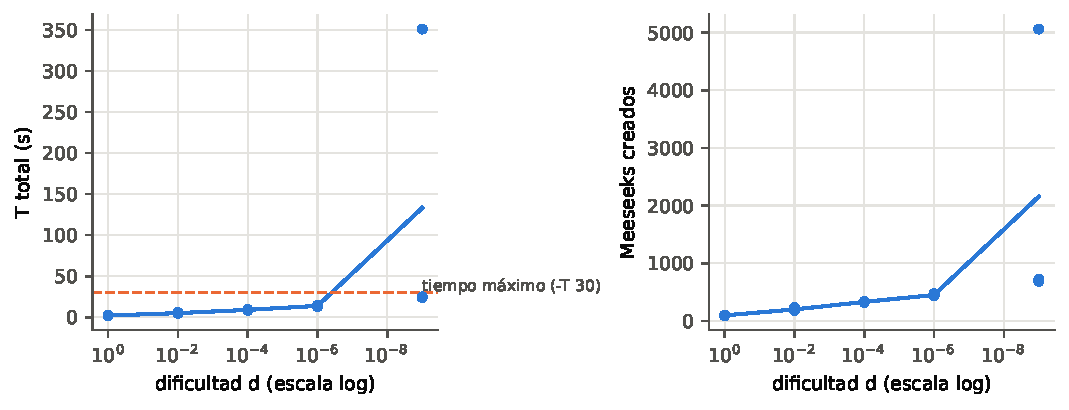
\includegraphics[width=\linewidth]{figs/e6_extra.pdf}
\caption{E6: tiempo total y Meeseeks creados para dificultades muy pequeñas.}
\end{figure}

\paragraph{Observaciones.}
\begin{itemize}[leftmargin=1.5em]
\item Mientras el sistema no se sature, el costo crece de forma logarítmica: cada factor de
  100 en la dificultad agrega unos 5 niveles y unos 4 a 5~s. Incluso $d=10^{-9}$ se resolvió
  en dos de tres corridas en unos 24~s, por debajo del máximo, con unos 700 Meeseeks.
\item La tercera corrida con $d=10^{-9}$ es el caso que pide el enunciado: superó los 30~s,
  se decretó el caos y, sin terminar el programa, la solución llegó a los 351~s, es decir,
  \textbf{321~s adicionales}. Lo notable es que la espera simulada del camino ganador fue de
  solo 22.5~s: casi todo el tiempo (328~s) fue tiempo real del sistema. Se crearon 5059
  Meeseeks, con 4543 vivos a la vez, que consumieron 579~s de CPU en dos núcleos.
\item La explicación es la misma que en E4b. Por azar, ese árbol creció más ancho que los
  otros; con miles de padres esperando un \emph{slot} y reintentando cada 25~ms, la CPU se
  satura en espera activa, los Meeseeks que sí trabajan se planifican tarde y el árbol
  avanza cada vez más lento, lo que a su vez deja más padres esperando. Es una
  retroalimentación positiva: pasado cierto tamaño, la tarea no se vuelve un poco más lenta,
  sino un orden de magnitud más lenta.
\item Conclusión de la prueba: el tiempo adicional que necesita una tarea muy difícil no es
  predecible a partir de su dificultad, porque depende de si el árbol cruza el umbral de
  saturación. Por debajo del umbral bastan segundos; por encima, varios minutos. Esto
  justifica que el tiempo máximo exista y que su acción sea terminar todo el grupo de
  procesos: seguir esperando puede costar mucho más que reintentar la solicitud.
\end{itemize}

A escala real (300~s de máximo y duraciones de 0.5 a 5~s) cada generación tarda en promedio
2.75~s en lugar de 0.25~s, por lo que el mismo árbol necesitaría unas 11 veces más tiempo
simulado: una tarea con $d=10^{-9}$ (unos 34 niveles) pasaría de los 300~s solo por las
esperas, aun sin saturación. Por esa razón la prueba se hizo a escala y no con los 5
minutos completos, que habrían requerido horas por corrida. La terminación por caos con un
tiempo máximo real se muestra en la corrida de la sección~\ref{sec:corridas}.
